\chapter{Definición y propiedades de los polinomios discretos de Legendre}
\label{cap: def de los pol de legendre discretos}

\section{Introducción: planteamiento y motivación}
Durante todo este trabajo trataremos con señales
finitas
(digamos, de
longitud $n$), y las pensaremos como elementos de $\IR^{n}$.
En la práctica, por lo general
una señal es un conjunto de mediciones tomadas
a intervalos regulares de tiempo.
Puesto que por el momento no vamos
a considerar la localización temporal, dicha
información perfectamente puede expresarse como 
una $n-$tupla. En lo que sigue, a menos que se diga
lo contrario, usaremos indistíntamente los nombres
``vector'' y ``señal'.'

Es costumbre empezar
a enumerar las entradas de un vector
de $x \in \IR^{n}$ a partir de uno, pero
para nuestros fines,
como se verá más adelante, es más 
conveniente empezar desde el cero.
Adoptamos pues esta convención.

\sidenote{\TODO{Di por qué prefieres
evitar el nombre ``'lineal'. Baja la nota a
la altura de la def.}}

\begin{defi}
\label{def: grafica senial}
Por la \textbf{gráfica de una señal} $x=(x_{j})_{j=0}^{n-1}$
de dimensión $n$ entenderemos
 el siguiente subconjunto de $\IR^{2}$:
\[
G_{x} := 
\{ (j, x_{j} ) : \hspace{0.1cm} 0 \leq j \leq n-1
\hspace{0.2cm} \text{entero}\} .
\]
Si $G_{x}$ está contenida en la gráfica de una recta, diremos que la
señal es \textbf{afín}
(en el caso particular en el que
la ecuación de la recta en cuestión sea de la forma $y= h$
(con $h$ una constante),
diremos que la señal es
\textbf{constante}). Si  $G_{x}$ está contenida en 
una parábola, o sea, en una
gráfica de ecuación cartesiana
$y=ax^{2}+ bx +c$, donde $a \neq 0$, diremos 
que la señal es \textbf{cuadrática}.
\end{defi}


\begin{figure}[H]
	\sidecaption{En la figura se pintan las gráficas
	de dos señales de dimensión 30. La gráfica de cruces 
	(resp. la de puntos)
	sugiere la forma de una recta (resp. una parábola).
	Tomamos a las formas de una parábola como cánones
	de curvas (y no, por ejemplo, trozos de circunferencias)
	sólo porque son buenos ejemplos de curvas con una sola 
	convexidad.}
	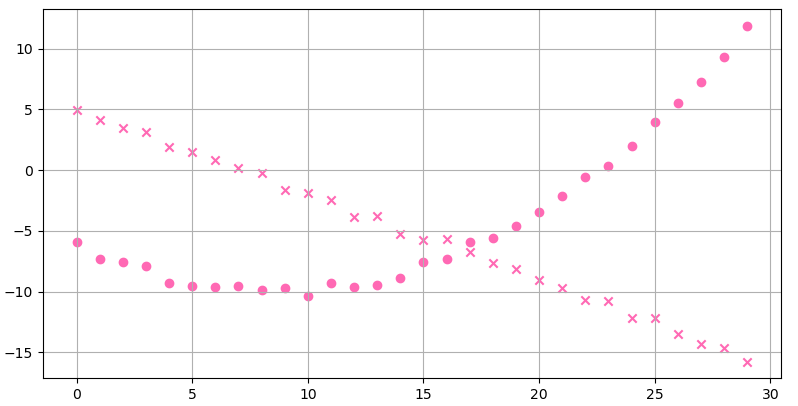
\includegraphics[scale=0.6]{ejemplo_intro} 
 \end{figure}

Puesto que el espacio subyacente de 
la teoría es el $\IR-$espacio vectorial 
$\IR^{n}$, tenemos la ventaja de contar con
bases (subconjuntos de $\IR^{n}$ linealmente
independientes y generadores de todo el espacio),
que pensamos en este contexto como sistemas
de representación: si 
\begin{equation}
\label{eq0: 13Feb}
\cali{B}=\{v_{k}
 \hspace{0.1cm} |
\hspace{0.1cm} 0 \leq k \leq n-1 \} 
\subseteq \IR^{n}
\end{equation}
es base del espacio, entonces, dado $x \in \IR^{n}$, 
\textbf{existe} \textbf{únicos} escalares
$a_{k} \in \IR$, con $0 \leq k \leq n-1$
tales que

\begin{equation}
\label{eq1: 13Feb}
x = \suma{k=0}{n-1}{a_{k}v_{k}};
\end{equation}
observe entonces que $x$ 
queda completamente determinado por los
números $a_{k}$. Si lo que nos interesa es
la forma de la gráfica de $x$, es natural preguntarse lo siguiente:

\begin{preg}
\label{preg: sist repr}
Si $\cali{B}$ es como en \eqref{eq0: 13Feb}, $x \in \IR^{n}$
y $a_{k}$ con $0 \leq k \leq n-1$ son como en 
\eqref{eq1: 13Feb}, ¿es posible establecer condiciones
necesarias y suficientes que deban cumplir los coeficientes
$a_{k}$ para que $x$ sea constante, afín o cuadrática?
\end{preg}

Después de un poco de reflexión, se llega a que la respuesta 
a la pregunta \ref{preg: sist repr} depende de la base
$\cali{B}$, y que por lo general la respuesta es negativa.
Observe además que, en la formulación de la pregunta,
se supone que para una señal $x$ se pudo dar
explícitamente a los coeficientes $a_{k}$ aunque,
en realidad,  esta es una suposición optimista.
A pesar de que la existencia y unicidad de tales
coeficientes está asegurada, el calcularlos
puede requerir el tener que resolver sistemas cuadrados
de ecuaciones con una cantidad de parámetros que
depende linealmente de $n$, sistemas que son computacionalmente
difíciles de resolver si $n$ es ``grande''.

\TODO{Poner algunos ejemplos}. Esto motiva la
creación de la siguiente lista de deseos.


\noindent 
\begin{listaObj}
\label{lista de objetivos}
Fijada una dimensión $n$, 
buscamos una base 
\begin{equation}
\label{eq1: 28Nov}
\cali{L}^{n}=\{ \cali{L}^{n,k} \hspace{0.1cm} |
\hspace{0.1cm} 0 \leq k \leq n-1  \} \subseteq \IR^{n} 
\end{equation}
del espacio vectorial
$\IR^{n}$ ``adecuada'' para la representación de señales
$x \in \IR^{n}$,
en el sentido que satisfaga
las siguientes condiciones: 

\begin{enumerate}
\item 
que
sea ortonormal, para poder hacer uso de todas
las bondades que conlleva 
trabajar con tales bases, 
bondades entre las que se encuentran
las que a continuación citamos.
\begin{itemize}
\item 
\textbf{\color{ameMorado}{(Los coeficientes de $x$ respecto
a $\cali{B}$ son muy fáciles de calcular, ...)}}
El poder no sólo dar explícitamente los coeficientes
de un vector respecto a la base, 
	\marginnote{Si $x \in \IR^{n}$ y $\cali{L}^{n}$ como en 
	\eqref{eq1: 28Nov} es BON de $\IR^{n}$, entonces identificamos a
	$x$ con los $n$ números  
	$a_{k}:= \langle x, \cali{L}^{n,k} \rangle$,
	$0 \leq k \leq n-1$.}
sino poder calcular a estos
de forma relativamente sencilla (a saber, vía productos punto,
c.f. \TODO{referencia del apéndice} ); si
\eqref{eq1: 28Nov} es ortonormal, entonces

\begin{equation}
\label{eq2: 13Feb}
x= \suma{k=0}{n-1}{a_{k}\cali{L}^{n,k}},
\hspace{0.2cm} \text{ donde } \hspace{0.2cm}
a_{k}= \langle x , \cali{L}^{n,k} \rangle.
\end{equation}
\item
\textbf{\textcolor{ameMorado}{(... dan información sobre el tamaño (norma) de $x$...)}}
El tener disponible una igualdad de tipo Parseval
(c.f. \TODO{referencia del apéndice}), igualdad que
relaciona de manera sencilla (de hecho, lineal)
el cuadrado de
la magnitud de una señal $x \in \IR^{n}$ (magnitud dada
gracias al producto punto definido en $\IR^{n}$)
con el cuadrado de las magnitudes de sus coeficientes
respecto a la base;

\[
||x||^{2}= \suma{k=0}{n-1}{|a_{k}|^{2}}.
\]

Esto es útil al momento
de intentar determinar
(de forma intuitiva) 
	\marginnote{
		Si $x':= \suma{k=0, }{n-1}{a_{k} \cali{L}^{n,k}}$
	y $|a_{i}|$ es un número ``cercano a cero'', entonces
	$||x '|| \approx ||x||$. Pensando en la norma de $x$ como
	la cantidad de información que tenía, parafraseamos esto
	como ``quitar coeficientes pequeños no hace que se
	pierda mucha información''	
	.}
la importancia 
de cierto vector de la base para describir a $x$.
También es bueno contar con esta igualdad
al momento de hacer procesos de síntesis,
es decir, de modificación de la señal
via cambios en sus coeficientes respecto
a un sistema de representación; si un coeficiente
$a_{k}$ es pequeño en magnitud, retirando el sumando
$a_{k} \cali{L}^{n,k}$ de \eqref{eq2: 13Feb}, 
estamos seguros de obtener
un vector $x'$ similar al vector original $x$
en magnitud.
\end{itemize}
\item \textbf{
\textcolor{ameMorado}{(...y sobre la forma de la
gráfica de $x$.)}} El que,
dada la expresión \eqref{eq2: 13Feb},
sea posible establecer
una relación sencilla entre \textbf{los coeficientes }
$a_{k}$
(en base a su tamaño y signo) y
\textbf{la forma de la gráfica de la señal}.
En particular, nos gustaría encontrar condiciones
necesarias y suficientes 
en términos de los coeficientes $a_{k}$ para determinar
si la gráfica de $x$ es afín o cuadrática.
Queremos pues que los coeficientes $a_{k}$
\textit{reflejen atributos geométricos de $x$};
de esta forma, 
\textbf{con herramientas del álgebra lineal lograremos cuantificar
la propiedad geométrica intuitiva de ``parecerse a''
una recta o una parábola.}
\end{enumerate} 

\end{listaObj}


\begin{comment}
Nuestro acercamiento es como sigue:
\end{comment}
Puesto que son las
formas básicas de recta y parábola las que nos interesa
capturar,
consideramos a las gráficas de las potencias básicas
\begin{equation}
\label{eq0: 8En}
f_{k}(t)= t^{k}, \hspace{0.4cm}
-1 \leq t \leq 1, \hspace{0.2cm}
 k \in \overline{\IN};
\end{equation}
restringiendo su dominio al intervalo $[-1,1]$.
Como las funciones
resultantes ya son elementos del 
espacio de Hilbert $L^{2}[-1,1]$ (c.f. \TODO{apéndice})
y, como las funciones \eqref{eq0: 8En} son linealmente
independientes en este espacio, ya tiene sentido realizar
en el espacio $L^{2}[-1,1]$  un proceso de ortogonalización
(por ejemplo, usando el procedimiento de Gram-Schmidt 
\ref{Teo:Gram-Schmidt}) para obtener bases ortonormales
de los subespacios de $L^{2}[-1,1]$ que estas potencias
básicas generan; obtenemos así una familia de polinomios 
\begin{equation}
\label{eq1: 8En}
P_{k}(t), \hspace{0.4cm}
-1 \leq t \leq 1, \hspace{0.2cm}
 k \in \overline{\IN},
\end{equation}
estando cada polinomio $P_{k}$ determinado unívocamente
por las $k$ condiciones de ortogonalidad
\[
\forall \hspace{0.1cm} 0 \leq m \leq k-1: \hspace{0.1cm}
\int_{-1}^{1}{P_{k}(t)P_{m}(t)} dt = 0
\]
y por la condición de normalización 
\[
\int_{-1}^{1}{P_{k}(t)^{2}} dt = 1.
\]
A los polinomios $P_{k}$ que resultan
se les conoce como \textbf{polinomios de Legendre}
\sidenote{Muchas veces
esta condición de normalización cambia; algunos 
prefieren tomar como condiciones de ortonormalización a 
\[
\int_{-1}^{1}{P_{k}(t)P_{m}(t)} dt = \frac{2 \delta_{km}}{2n+1}.
\]
Por eso las fórmulas que usualmente uno encuentra para
los polinomios de Legendre (por ejemplo \TODO{Wikipedia})
son distintas a las presentadas aquí. \TODO{Pero son múltiplos
escalares?}} (c.f. \cite{friedberg} , p.346).

Se calcula fácilmente que los primeros cuatro 
polinomios de Legendre son

\[
P_{0}(t) = 1/\sqrt{2},
\]

\[
P_{1}(t) = \sqrt{\frac{3}{2}}t,
\]

\[
P_{2}(t) = \sqrt{\frac{5}{8}}\left( 3t^{2}-1 \right),
\]
y
\[
P_{3}(t) = \frac{5}{2} \sqrt{\frac{7}{2}}\left( t^{3}- \frac{3}{5}t\right).
\]

Puesto que el conjunto de los polinomios de Legendre
definidos arriba es una base ortonormal del
espacio $L^{2}([-1,1])$
\sidenote{\TODO{Agrega las correspondientes 
referencias al apéndice.}}
(c.f. \cite{DSML} p.390), una función definida
en el intervalo $[-1,1]$ puede aproximarse
``tanto como se quiera'' en base a combinaciones
lineales de polinomios de Legendre.


Si planeamos, de alguna forma, usar a estos polinomios
para el estudio morfológico de señales, por la naturaleza
discreta de estos últimos objetos, será
inevitable realizar, en algún punto 
del argumento, un proceso discretización
(por ejemplo, 
via una discretización
puntual, c.f definición \TODO{ref}), es decir,
pasar del ``contexto continuo'' en el que se han
definido los polinomios de Legendre a uno discreto.

Para partir de
objetos en el espacio ambiente
$\IR^{n}$ de nuestro interés,
también tiene sentido primero realizar
un proceso de discretización (por ejemplo, 
puntual) y luego realizar
un proceso de ortogonalización. La figura
\ref{fig: ortogonalizacion, discretizacion}
ilustra, para el caso $n=4$, estos dos caminos.
Como ahí se aprecia, estos dos caminos llevan 
a resultados distintos. Sin embargo, puesto que lo
que interesa es tener condiciones de ortogonalidad
en el espacio $\IR^{n}$, es obvio que 
el camino a seguir debe ser uno parecido al segundo.


Escogida pues la opción de primero 
discretizar polinomios para posteriormente
ortonormalizar, queda todavía abierta
la decisión de qué método de discretización usar.

Elegimos empezar
con discretizaciones puntuales de polinomios.
En base a estos objetos lograremos definir
una base ortonormal de $\IR^{n}$ que cumple satisfactoriamente
los requisitos explicados en la lista de deseos
\ref{lista de objetivos}, y a la que llamaremos
la \textbf{base de Legendre discreta de dimensión $n$}.

Un segundo punto de vista, basado
en discretizaciones por promedios integrales,
se presentará después en
\ref{Construcción de Ln en base a discretizaciones con sumas integrales}; 
como demostraremos a lo largo del capítulo, 
ambas alternativas
de discretización, igual de naturales la una que la otra, nos
conducen a la misma base ortonormal de $\IR^{n}$,
que, como se ilustra en la subsección de ejemplos
\ref{subsec: ejemplos}
resulta ser un sistema de representación
realmente útil para el estudio morfológico de señales finitas.

\newpage %Nueva página para la figura enorme que sigue.

\begin{figure}[H]
\centering\captionsetup{format = hang}
	\begin{measuredfigure}
		\label{fig: ortogonalizacion, discretizacion}
		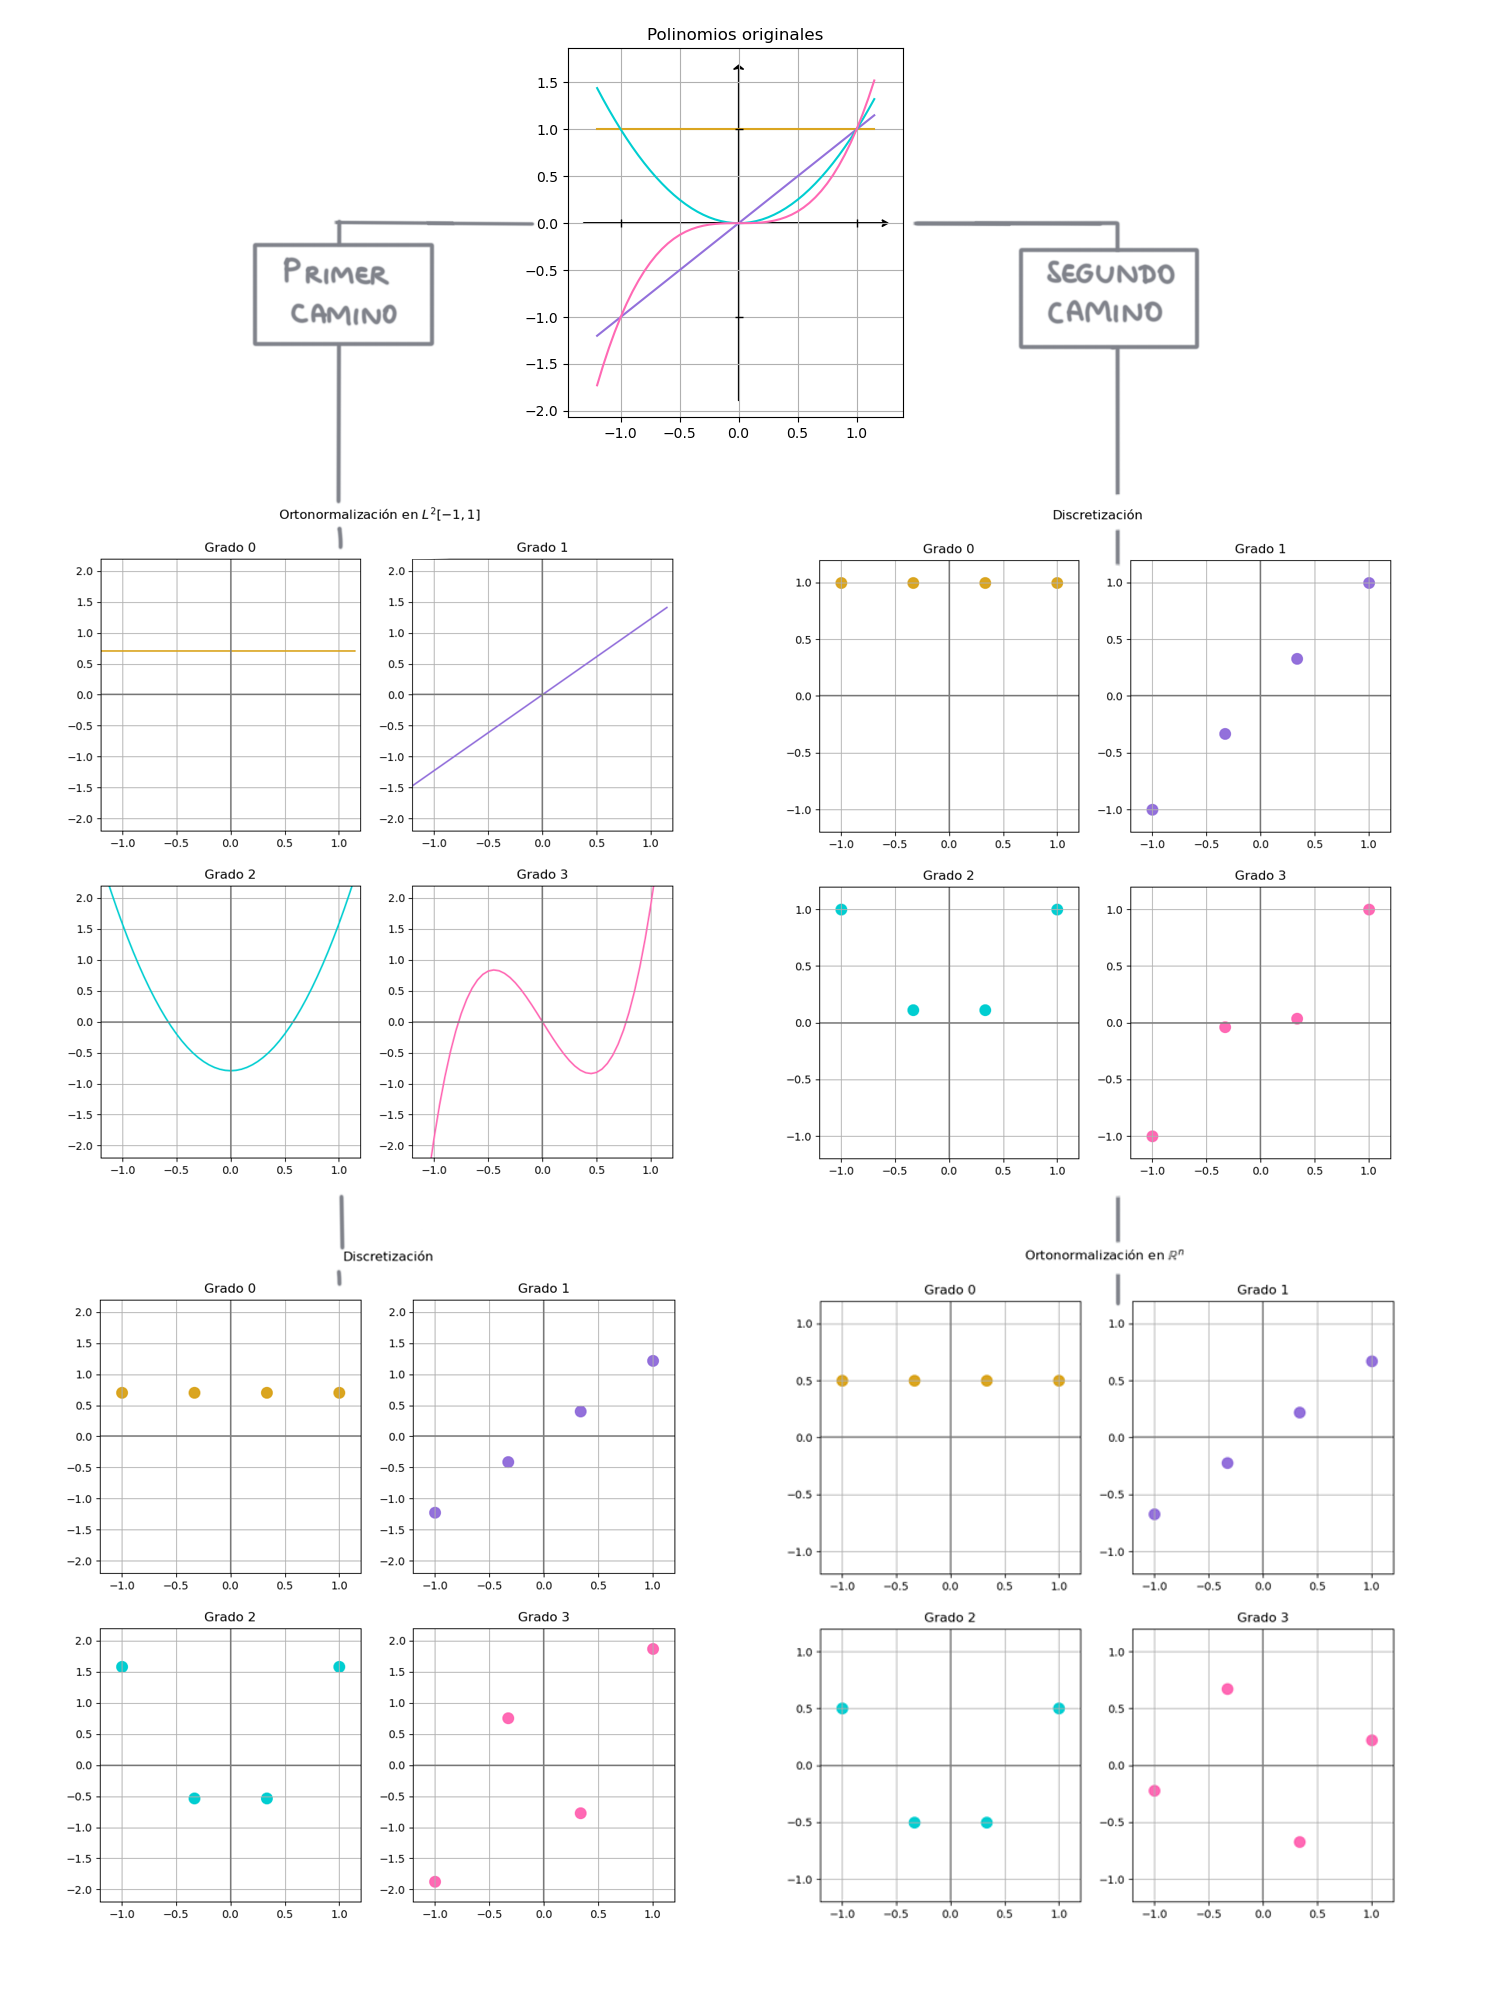
\includegraphics[scale=1.3]{discr_ortog} 
		\caption{Como se aprecia, las operaciones de
		ortogonalización y discretización no son conmutativas.}
 	\end{measuredfigure}
 \end{figure}